\documentclass[conference]{IEEEtran}
\IEEEoverridecommandlockouts{}
\usepackage[letterpaper, top=50pt, left=54pt, right=54pt, bottom=58pt]{geometry}
\usepackage{cite}
\usepackage{amsmath,amssymb,amsfonts}
\usepackage{algorithmic}
\usepackage{graphicx}
\usepackage{textcomp}
\usepackage{xcolor}
\usepackage{hyperref}
\usepackage{float}
%% ODE handling
\usepackage{diffcoeff}
\usepackage{booktabs}
%% The SI units alignment
\usepackage{siunitx}
\usepackage{relsize}
\setlength\abovedisplayskip{2.5pt}
\setlength\belowdisplayskip{2.5pt}
\setlength{\textfloatsep}{2.5pt}
\setlength{\intextsep}{2.5pt}

\def\BibTeX{{\rm B\kern-.05em{\sc i\kern-.025em b}\kern-.08em
 T\kern-.1667em\lower.7ex\hbox{E}\kern-.125emX}}
\newcommand{\ui}[2]{#1_{\mathrm{#2}}}
\newcommand{\uis}[2]{#1^{\mathrm{#2}}}
\newcommand{\coo}{\ensuremath{\mathrm{CO_2}}}
\newcommand{\chho}{\ensuremath{\mathrm{CH_2O}}}
\newcommand{\citep}{\cite}

\begin{document}

\title{\vspace*{18pt}Carbon Neutral Greenhouse: Economic Model Predictive Control Framework for Education
    \thanks{The authors acknowledge the support of the Program to support young researchers at STU under the project AIOperator: eXplainable Intelligence for Industry, as well as the contribution of the Scientific Grant Agency of the Slovak Republic under the grants 1/0490/23 and 1/0297/22. This research is funded by the Horizon Europe under the grant no. 101079342 (Fostering Opportunities Towards Slovak Excellence in Advanced Control for Smart Industries). RP acknowledges the financial support by the European Commission under the grant scheme NextGenerationEU project no. 09I03-03-V04-00530.}
}

\author{\IEEEauthorblockN{Marek Wadinger, Rastislav F\'aber, Erika Pavlovi\v cov\'a, Radoslav Paulen}
    \IEEEauthorblockA{\textit{Faculty of Chemical and Food Technology,}
        \textit{Slovak University of Technology in Bratislava,}
        \textit{Bratislava, Slovakia} \\
        \texttt{marek.wadinger@stuba.sk}}
}

\maketitle

\begin{abstract}
    This paper presents a comprehensive framework aimed at enhancing education in modeling, optimal control, and nonlinear Model Predictive Control (MPC) through a practical greenhouse climate control model. The framework includes a detailed mathematical model of lettuce growth and greenhouse environment, which are influenced by real-time external weather conditions obtained via an application programming interface (API). Using this data, the MPC-based approach dynamically adjusts greenhouse conditions, optimizing plant growth and energy consumption and minimizing the social cost of CO\textsubscript{2}. The presented results demonstrate the effectiveness of this approach in balancing energy use with crop yield and reducing CO\textsubscript{2} emissions, contributing to economic efficiency and environmental sustainability.
    The framework also provides a valuable resource for making control systems education more engaging and effective. The main aim is to provide students with a hands-on platform to understand the principles of modeling, the power of MPC and the trade-offs between profitability and sustainability in agricultural systems. The framework gives students a hands-on experience, helping them to understand the control theory better, connecting it to the practical implementation, and developing their problem-solving skills. It can be accessed at \url{ecompc4greenhouse.streamlit.app}.
\end{abstract}

\begin{IEEEkeywords}
    Control education, Computer aided learning, Predictive control for nonlinear systems
\end{IEEEkeywords}

\section{Introduction}
In the evolving field of engineering, graduates must possess both theoretical knowledge and practical skills. Technical university education should therefore combine a solid theoretical foundation with hands-on experiences, gained through projects, real-world problem solving, and experimentation. Interactive tools have proven valuable for teaching control theory~\cite{Emami1991, Guzman2013}, and importantly, practical learning need not depend on costly laboratory setups—simulations and interactive tasks can provide effective, accessible alternatives.

Modern agriculture remains labor-intensive, seasonal, and heavily reliant on irrigation and subsidized inputs, often resulting in eutrophication, deforestation, and soil degradation. With nearly 70\% of global water use attributed to agriculture~\cite{Debroy2024}, greenhouses offer a promising alternative by creating controlled environments that enhance productivity beyond conventional farming. However, internal climate fluctuations remain a challenge, requiring efficient control strategies~\cite{Wu2019}.

Solar radiation is central to greenhouse productivity. Key metrics include Global Horizontal Irradiance (GHI) and Photosynthetically Active Radiation (PAR), the latter directly influencing photosynthesis. Recent studies have reviewed empirical models estimating PAR from GHI~\cite{NoriegaGardea2021}. To improve prediction accuracy, hybrid modeling addresses missing data, while Machine Learning (ML) techniques adapt to dynamic conditions~\cite{Iddio2020, MaLu2022}. Deep learning methods have also been used to forecast plant growth from time-series data~\cite{Yasrab2021}.

Several control strategies have been explored to improve greenhouse performance. Adaptive control reacts to real-time changes~\cite{Tian2022}; nonlinear feedback~\cite{Bood2023}, fuzzy logic~\cite{smartcities7030055}, robust~\cite{Zhang2021}, and optimal control~\cite{Debroy2024, SVENSEN2024108578} offer various benefits in handling complexity and uncertainty. However, these methods often involve complex implementation and frequent tuning, potentially increasing energy use and mechanical wear. While PID controllers remain common due to their simplicity, they require multiple units and extensive tuning. Recent approaches combining PID with IoT and ML~\cite{Wang2024} offer improvements, but often lack optimality guarantees. As a result, Model Predictive Control (MPC) is increasingly favored for its ability to optimize setpoints continuously via online sample-by-sample updates~\cite{Hu2022}.

While PID controllers are valued for their simplicity and effectiveness, IoT and ML are also being integrated into greenhouse control, as demonstrated by~\cite{Wang2024}, who combined these technologies with PID for real-time monitoring. Nonetheless, managing greenhouse systems using PID can be challenging due to the need for multiple controllers and extensive tuning. This process is time-consuming and case-dependent, often lacking guaranteed optimal results. Consequently, MPC has emerged as a preferred approach for greenhouse climate control~\cite{Hu2022}, enabling continuous adjustment of setpoints through sample-by-sample online optimization.

In parallel, integrating advanced control techniques into education has gained attention. Web-based simulation platforms have been shown to improve student engagement and bridge the gap between theory and practice~\cite{WangEducation2024, Zakova2024}. This work contributes to that goal by presenting a framework for greenhouse climate control that emphasizes modeling, optimal control, and Nonlinear Economic MPC (NEMPC).

Specifically, we present a web interface for optimal greenhouse climate control, designed to enhance crop yield, energy efficiency, and reduce \coo\ emissions. Using principles of thermodynamics, fluid dynamics, and mass transfer—alongside real-time weather and carbon intensity forecasts—we developed a simulation environment where NEMPC dynamically adjusts ventilation, heating, humidification, and \coo\ enrichment. Beyond its technical contributions, the framework serves as an educational platform, enabling students to explore economic and sustainability trade-offs in agricultural systems.

\section{Greenhouse Climate Model}
\label{sec:greenhouse}
This section outlines the mathematical greenhouse model implemented within the GES software~\cite{Ward2019} based on the Gembloux Dynamic Greenhouse Climate Model~\cite{Mashonjowa2007} and the work by Vanthoor~\cite{Vanthoor2011}. The model captures wind, temperature, humidity, and \coo\ concentration dynamics. For the complete list of parameters and values with references, see the source code repository\footnote{\url{https://github.com/MarekWadinger/ecompc-greenhouse-platform/blob/main/core/greenhouse_model.py}}.
\begin{figure}
    \centering
    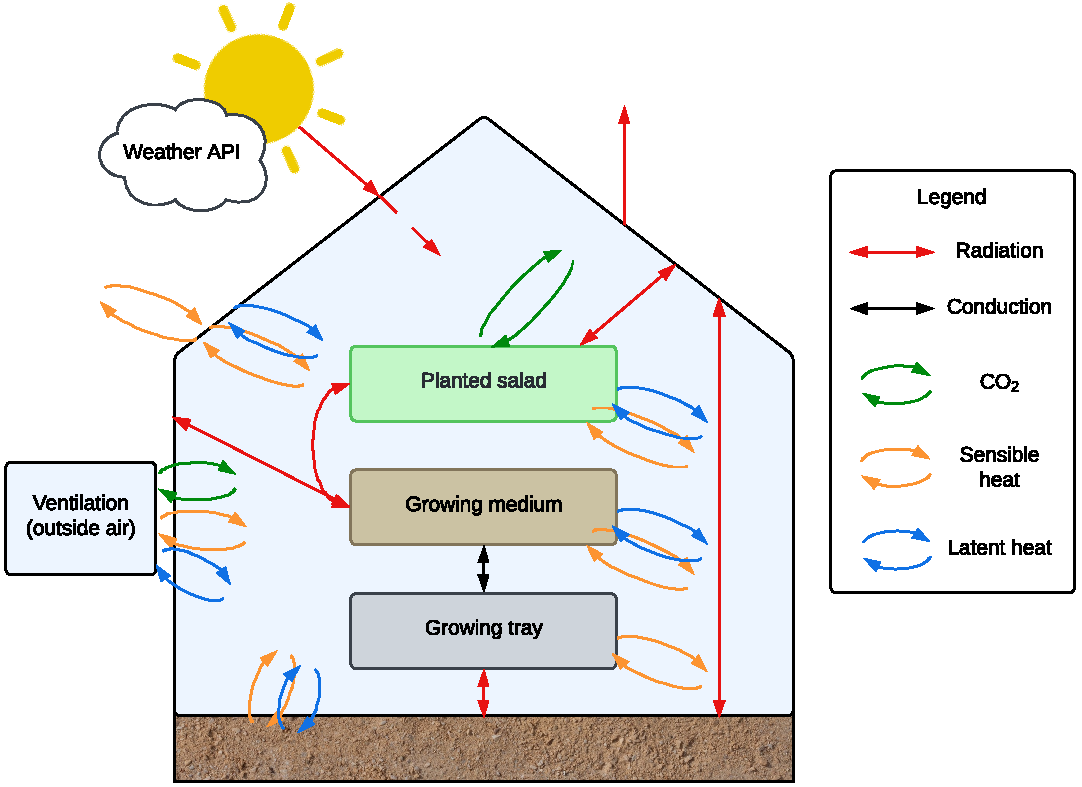
\includegraphics[width=\linewidth]{figures/diagramGH.pdf}
    \caption{Simplified diagram of heat, mass, and \coo\ in the model. Adapted from~\cite{Ward2019}.}\label{fig:diagram}
\end{figure}

\subsection{Temperature Dynamics}\label{subsec:temperature}

The temperature evolution is governed by convection, radiation, and conduction between different compartments (cover, internal air, vegetation, tray, etc.), as illustrated in Fig.~\ref{fig:diagram}.
Convective, radiative, and conductive heat transfers are modeled using standard correlations involving Nusselt, Reynolds, and Grashof numbers. For brevity, detailed equations are omitted here but can be found in~\cite{Ward2019,Vanthoor2011}.

% The convective heat transfer between two surfaces reads as:
% \begin{equation}
%     \text{Nu} = \max \left( \text{Nu}_G, \text{Nu}_R \right),
% \end{equation}
% where \(\text{Nu}_G\) and \(\text{Nu}_R\) are the Nusselt numbers for free and forced convection, respectively:
% \begin{align}
%     \text{Nu}_G & = 0.5  {\left( \frac{\text{Gr}}{10^5} \right)}^{0.25} + 0.13  {\left(\frac{\text{Gr}}{10^5}\right)}^{0.33}, \\
%     \text{Nu}_R & = 0.6  {\left(\frac{\text{Re}}{20000}\right)}^{0.5} + 0.032  {\left(\frac{\text{Re}}{20000}\right)}^{0.8},
% \end{align}
% where Re represents the Reynolds number, and Gr represents the Grashof number. The convective heat flux is then:
% \begin{equation}
%     Q_{\text{conv}} = A_{\text{c}}\, \text{Nu}\, \lambda_{\text{air}} \frac{T_1 - T_2}{d_{\text{c}}},
% \end{equation}
% where \(A_c\) and \(d_c\) represent the characteristic area and length of a compartment, respectively, and \(\lambda_{air}\) is the approximate air thermal conductivity at room temperature.

% The radiative heat transfer is described by:
% \begin{equation}
%     Q_{\text{rad}} = \frac{\varepsilon_1  \varepsilon_2}{1 - \rho_1  \rho_2  F_{12}  F_{21}}  \sigma  A_1  F_{12}  \left( T_1^4 - T_2^4 \right),
% \end{equation}
% where \(\sigma \) is the Stefan-Boltzmann constant, \(F_{12}\) is the view factor from surface 1 to surface 2, \(T_1\) and \(T_2\) represent the temperatures of the surfaces, and \(\varepsilon \) and \(\rho \) are the emissivity and reflectivity of the surfaces, respectively.

% The conductive heat transfer through a medium is given by:
% \begin{equation}
%     Q_{\text{cond}} = \frac{A \lambda_{\text{c}}}{d_\text{l}} (T_1 - T_2),
% \end{equation}
% where \(\lambda_{\text{c}} \) is the thermal conductivity of a compartment, and \(d_{\text{l}}\) is the thickness of the conducting layer.

\subsection{Humidity Dynamics}\label{subsec:humidity}

Humidity is modeled through vapor mass transfer, where the air moisture content depends on air temperature and pressure. The density of water vapor follows an empirical exponential relation given by:
\begin{equation}
    \ui{C}{w} = \ui{\rho}{air} \exp^{11.56 - \frac{4030}{T + 235}},
\end{equation}
where \(\ui{\rho}{air}\) is the density of air.

% The mass transfer of water vapor due to convection is:
% \begin{equation}
%     Q_{v} = \frac{A  H_{\text{fg}}}{\rho  c}  \frac{\text{Sh}}{\text{Le}}  \frac{\lambda}{d}  \left( C - C_{\text{sat,}T} \right),
% \end{equation}
% where \(H_{\text{fg}}\) is the latent heat of vaporization, \(\text{Sh}\) is the Sherwood number, and \(\text{Le}\) is the Lewis number, \(\lambda \) is the thermal conductivity, \(d\) is the characteristic length, \(A\) is the heat exchange surface area, \(\rho \) is the density of the vapor, \(c\) is the specific heat capacity, \(C\) is the actual vapor concentration --- referring  to the amount of water vapor present in the air in a given volume --- and \(C_{\text{sat,}T}\) is the saturated vapor concentration at temperature \(T\).

\subsection{Carbon Dioxide Concentration Dynamics}

The \coo\ concentration is affected by photosynthesis and external conditions. The external \coo\ concentration is computed as:
\begin{equation}
    \ui{C}{\coo,ext} = \frac{4 \times 10^{-4}  M_{\coo}  \ui{P}{atm}}{R  \ui{T}{ext}},
\end{equation}
where \(M_{\coo}\) is the molar mass of \coo, \(\ui{P}{atm}\) is the atmospheric pressure, \(R\) is the gas constant, and \(\ui{T}{ext}\) is the external air temperature in Kelvin.

The internal \coo\ concentration in ppm is given by:
\begin{equation}
    \ui{C}{\coo, ppm} = \frac{C_{\coo}  R  \ui{T}{i}}{M_{\coo}  \ui{P}{atm}} \times 10^6,
\end{equation}
where \(C_{\coo}\) is the \coo\ density, and \(\ui{T}{i}\) is the internal air temperature in Kelvin.

The greenhouse climate model integrates the models of temperature, humidity, and \coo\ concentration into a dynamic system represented by a state vector \linebreak \(x\) = [\(\ui{T}{c}, \ui{T}{i}, \ui{T}{v}, \ui{T}{m}, \ui{T}{p}, \ui{T}{f}, \ui{T}{s}, \ui{C}{w}, \ui{C}{\coo}, \ui{x}{sdw}, \ui{x}{nsdw}\)] \( \in\mathbb R^{11} \), and input vector \(u\) = [\(\ui{Q}{heater}, \ui{R}{fan}, \ui{V}{humid}, \ui{G}{\coo} \)] \( \in\mathbb R^{4} \) for the heating power, ventilation, humidification, and \coo\ enrichment. The \(\ui{T}{c}\) represents the cover temperature, \(\ui{T}{i}\) the internal air temperature, \(\ui{T}{v}\) the plant temperature, \(\ui{T}{m}\) the growing medium temperature, \(\ui{T}{p}\) the tray temperature, \(\ui{T}{f}\) the floor temperature, and \(\ui{T}{s}\) the temperature of the soil layer. Additionally, \(\ui{x}{sdw}\) denotes the structural dry weight of the plant and \(\ui{x}{nsdw}\) the non-structural dry weight of the plant.

The model is influenced by external conditions \linebreak \( p = \left[
    \ui{T}{ext}, \ui{T}{app}, \ui{v}{wind}, \ui{H}{rel}, \ui{\mathbf{I}}{POA,dir}, \ui{\mathbf{I}}{POA,diff} \right] \in \mathbb{R}^{20} \) denoted as \(p\). The \(\ui{T}{app}\) represents the apparent temperature, \(\ui{v}{wind}\) is the wind speed, \(\ui{H}{rel}\) the relative humidity, and \(\ui{\mathbf{I}}{POA,dir}\in \mathbb{R}^{8}\) and \(\ui{\mathbf{I}}{POA,diff}\in \mathbb{R}^{8}\) represent the plane of array (POA) direct and diffuse solar radiation, respectively. Additionally, \(\ui{\mathbf{I}}{POA,dir}\) and \(\ui{\mathbf{I}}{POA,diff}\) from all planes of the greenhouse are integrated, providing a realistic and dynamic input for the control strategy.

\subsection{Actuation Control Systems}
Actuators translate MPC signals into mechanical actions to regulate environmental variables~\cite{Butterfield2018}. Table~\ref{tab:actuators} summarizes the actuated variables. We monitor each actuator's contribution to the overall energy balance, operating costs, and \coo\ emissions.
\begin{table}
    \centering
    \caption{Actuator Model Parameters}\label{tab:actuators}
    \begin{tabular}{lcc}
        \toprule
        Actuator        & Label                & Unit                   \\
        \midrule
        Heater          & \( \ui{Q}{heater} \) & W                      \\
        Fan             & \( \ui{R}{fan} \)    & m\textsuperscript{3}/s \\
        Humidifier      & \( \ui{V}{humid} \)  & l/h                    \\
        \coo\ Generator & \( \ui{G}{coo} \)    & kg/h                   \\
        \bottomrule
    \end{tabular}
\end{table}
We model the actuators by adjusting the control signal, \( u(t) \), which ranges from 0 to 100\%, where 0\% and 100\% corresponds to no actuation and maximum actuation, respectively. The actuation level, \( a(u) \), is then calculated as:
\begin{equation}
    a(u) = \frac{u}{100}  \ui{a}{max},
\end{equation}
where \( \ui{a}{max} \) represents the maximum of the specific actuator.

The power consumption of an actuator is determined by:
\begin{equation}
    P(u) = \frac{\ui{p}{unit}}{\eta}  a(u),
\end{equation}
where \( \ui{p}{unit} \) is the power per unit of actuation, and \( \eta \) represents the efficiency of the actuator.

The total energy cost in EUR is calculated as:
\begin{equation}
    \ui{C}{energy}(u) = \frac{\ui{E}{cost}  \Delta t}{1000 \times 3600}  P(u),
\end{equation}
where \( \ui{E}{cost} \) is the cost of energy in EUR per kWh, and \( \Delta t \) is the time step in seconds.

The \coo\ emissions generated by an actuator are given by:
\begin{equation}
    \ui{E}{\coo}(u) = \frac{\ui{I}{\coo}  \Delta t}{1000 \times 3600}  P(u),
\end{equation}
where \( \ui{I}{\coo} \) represents the carbon intensity~\cite{ElectricityMaps2022}, measured in g\coo{}eq/kWh. The associated cost of these emissions is:
\begin{equation}
    \ui{C}{\coo}(u) = \ui{C}{\coo,cost}  \ui{E}{\coo}(u),
\end{equation}
where \( \ui{C}{\coo,cost} \) is the social cost of \coo\ in EUR/g\coo\ eq.

The heating power is determined based on the temperature setpoint, \( \ui{T}{sp} \), and air volume of the greenhouse, \( \Omega \), as:
\begin{equation}
    \ui{Q}{heater} = \ui{\rho}{air}  \ui{c}{air}  \Omega  (\ui{T}{sp} - \ui{T}{i})  \frac{\ui{Q}{air}}{3600},
\end{equation}
where \( \ui{\rho}{air} \) is the air density, \( \ui{c}{air} \) is the air specific heat capacity, and \( \ui{Q}{air} \) represents the fresh air exchange rate.

The ventilation rate, \( \ui{R}{fan} \), is based on air changes per hour (\( \text{ACPH} \)) --- the number of times the air in a space is replaced in an hour --- and greenhouse volume \( \Omega \):
\begin{equation}
    \ui{R}{fan} = \Omega \frac{\text{\( \text{ACPH} \)}}{3600}.
\end{equation}

The humidification rate, \( \ui{V}{humid} \), is calculated as:
\begin{equation}
    \ui{V}{humid} = \Omega \frac{\ui{\phi}{a, 80 - 40}}{\ui{\rho}{water}},
\end{equation}
where and \( \ui{\rho}{water} \) is the water density and  \( \ui{\phi}{a, 80 - 40} \) is the maximum change in absolute humidity per hour which corresponds to difference between the absolute humidity at 80\% and 40\% relative humidity at a temperature of 20\( ^\circ \)C.

The \coo\ generation is based on the desired change rate of the \coo\ density, \( \ui{\dot{C}}{\coo} \) in the greenhouse as:
\begin{equation}
    G_{\coo} = \ui{\dot{C}}{\coo} \Omega.
\end{equation}

\section{Plant Growth Model}\label{sec:lettuce_growth}
The growth of plant is modeled using a dynamic system of equations that captures the behavior of both structural (SDW) and non-structural dry weight (NSDW) of the plant~\cite{VANHENTEN199455}. The dynamics of the model is influenced by environmental factors such as temperature, light (PAR), and \coo\ concentration. The model equations are parameterized using well-established constants from the literature and adapted for dynamic simulation. For the complete list of parameters and their values with references, see source code repository\footnote{\url{https://github.com/MarekWadinger/ecompc-greenhouse-platform/blob/main/core/lettuce_model.py}}.

\subsection{Growth Dynamics} The rate of change of structural dry weight is governed by the specific growth rate \( \ui{r}{gr} \) and is modeled as:
\begin{equation}
    \diff{\ui{x}{sdw}}{t} = \ui{r}{gr}(\ui{T}{i}) \ui{x}{sdw}.
\end{equation}
Similarly, the rate of change of non-structural dry weight is given by:
\begin{equation}
    \diff{\ui{x}{nsdw}}{t} = c_{\eta} \ui{f}{phot}(\ui{C}{\coo}, \ui{T}{i}) - \gamma \ui{r}{gr}(\ui{T}{i}) \ui{x}{sdw} - \ui{f}{resp}(\ui{T}{i}),
\end{equation}
where \( c_{\eta} \) is the conversion factor representing the efficiency of absorbed carbon dioxide conversion into biomass (\(\mathsmaller{\chho/\coo}\)), \( \ui{f}{phot} \) is the gross photosynthesis rate, and \( \ui{f}{resp} \) is the maintenance respiration rate. Using \( Y_{\eta} \) as the yield, the coefficient \( \gamma \) accounts for biomass partitioning and respiratory losses, defined as \( \gamma = 1 + (1 - Y_{\eta}) / Y_{\eta} \).

\subsection{Specific Growth Rate} The specific growth rate \( \ui{r}{gr} \) describes the accumulation rate of the structural biomass (SDW) in response to the available non-structural dry weight (NSDW). This process is temperature-dependent and scales based on plant temperature sensitivity. The NSDW provides a reservoir of energy for structural growth. The efficiency of the energy conversion is central to the plant's overall biomass accumulation.

\subsection{Maintenance Respiration} The maintenance respiration rate \( \ui{f}{resp} \) accounts for the energy expenditure required to sustain the plant basic metabolic functions. The respiration process is divided between the shoot and root components, each with its own maintenance respiration rate, scaled to the plant dry mass. Respiration demands increase as temperature rises. It is a key factor in determining the amount of energy for growth as it consumes a portion of the energy generated from photosynthesis.

\subsection{Gross Photosynthesis} The gross canopy photosynthesis rate \( \ui{f}{phot} \) represents the total \coo\ assimilation by the plant. This is primarily driven by the maximum \coo\ assimilation rate, which depends on incident PAR, \coo\ concentration, and canopy light-use efficiency. The leaf area index and extinction coefficient further influence the efficiency of light absorption across the canopy. Canopy conductance plays a critical role in this process by regulating the rate at which \coo\ diffuses into the leaf. The combined effect of boundary layer conductance, stomatal conductance, and carboxylation conductance ensures that \coo\ reaches the sites of photosynthesis efficiently. Carboxylation conductance is temperature-dependent, reflecting the enzymatic activity affected by ambient conditions.
%
% \subsection{Specific Growth Rate}

% The specific growth rate \( \ui{r}{gr} \) is defined as:

% \begin{equation}
%     \ui{r}{gr} = \ui{c}{gr, max} \frac{\ui{x}{nsdw}}{\ui{c}{\gamma} \ui{x}{sdw} + \ui{x}{nsdw}} \ui{c}{qr, Q10}^{\left(\frac{\ui{u}{T} - 20}{10}\right)}
% \end{equation}

% where \( \ui{u}{T} \) is the canopy temperature, \( \ui{c}{gr, max} \) is the saturated growth rate at 20°C, \( \ui{c}{\gamma} \) is the growth rate coefficient, and \( \ui{c}{qr, Q10} \) is the growth sensitivy to change in temperature by 10\( ^\circ \)C.

% \subsection{Respiration Model}

% The maintenance respiration rate \( \ui{f}{resp} \) is defined as:

% \begin{equation}
%     \ui{f}{resp} = \left( \ui{c}{resp, s} (1 - \ui{c}{\tau}) \ui{x}{sdw} + \ui{c}{resp, r} \ui{c}{\tau} \ui{x}{sdw} \right) \ui{c}{resp, Q10}^{\left( \frac{\ui{u}{T} - 25}{10} \right)}
% \end{equation}

% where the \( \ui{c}{resp, s} \) and \( \ui{c}{resp, r} \) are the shoot and root maintenance respiration rate at 25°C, \( \ui{c}{\tau} \) is the root dry mass ratio, and \( \ui{c}{qr, Q10} \) is the respiration sensitivy to change in temperature by 10\( ^\circ \)C.

% \subsection{Photosynthesis Model}

% The photosynthesis model is divided into two parts: the maximum \coo\ assimilation rate and the gross canopy photosynthesis. The maximum \coo\ assimilation rate \( \ui{f}{phot, max} \) is given by:

% \begin{equation}
%     \ui{f}{phot, max} = \frac{\epsilon \ui{u}{PAR} \ui{g}{\coo} \ui{c}{\omega} (\ui{u}{\coo} - \Gamma)}{\epsilon \ui{u}{PAR} + \ui{g}{\coo} \ui{c}{\omega} (\ui{u}{\coo} - \Gamma)}
% \end{equation}

% where the \( \ui{u}{PAR} \) is the incident photosynthetically active radiation, \( \ui{u}{\coo} \) is the \coo\ concentration, \( \epsilon \) is the light-use efficiency, \( \ui{g}{\coo} \) is the canopy conductance to \coo\ diffusion, \( \ui{c}{\omega} \) is the density of \coo\ in air, and \( \Gamma \) is the \coo\ compensation point.

% The gross canopy photosynthesis \( \ui{f}{phot} \) is expressed as:

% \begin{equation}
%     \ui{f}{phot} = \left( 1 - \exp\left( -\ui{c}{K} \ui{c}{LAR} (1 - \ui{c}{\tau}) \ui{x}{sdw} \right) \right) \ui{f}{phot, max}
% \end{equation}

% where \( \ui{c}{K} \) is the extinction coefficient, and \( \ui{c}{LAR} \) is the structural leaf area ratio.

% \subsection{Canopy Conductance}

% The canopy conductance to \coo\ diffusion \( \ui{g}{\coo} \) is given by:

% \begin{equation}
%     \ui{g}{\coo} = \frac{1}{\left( \frac{1}{\ui{g}{BND}} + \frac{1}{\ui{g}{STM}} + \frac{1}{\ui{g}{CAR}} \right)}
% \end{equation}

% where \( \ui{g}{BND} \) is the boundary layer conductance, \( \ui{g}{STM} \) is the stomatal resistance, and \( \ui{g}{CAR} \) is the carboxylation conductance,

% \subsection{Carboxylation Conductance}

% The carboxylation conductance \( \ui{g}{CAR} \) is modeled as a quadratic function of temperature:

% \begin{equation}
%     \ui{g}{CAR} = \ui{c}{CAR1} \ui{u}{T}^2 + \ui{c}{CAR2} \ui{u}{T} + \ui{c}{CAR3}
% \end{equation}

% where:
% - \( \ui{c}{CAR1} \), \( \ui{c}{CAR2} \), and \( \ui{c}{CAR3} \) are carboxylation parameters dependent on temperature.
%
\section{Nonlinear Economic Model Predictive Control}\label{sec:mpc}
The NEMPC is adopted to maximize the profit of growing lettuce in a greenhouse by maximizing lettuce yield and minimizing operating costs over a finite prediction horizon. The NEMPC framework incorporates the dynamics of the greenhouse and time-varying external conditions.

\subsection{System Dynamics}\label{subsec:mpc_dynamics}
The greenhouse system dynamics is modeled by a set of nonlinear equations (see Sections~\ref{sec:greenhouse} and~\ref{sec:lettuce_growth}) summarized as:
\begin{equation}
    x(k+1) = f\left( x(k), u(k), p(k) \right),
\end{equation}
where, at time step \(k\), \(x(k) \in \mathbb{R}^{n_x}\) represents the state vector, \(u(k) \in \mathbb{R}^{n_u}\) is the control input vector (actuators), and \(p(k)\) are time-varying parameters, i.e., external climate conditions.

\subsection{Economic Objective Function}\label{subsec:mpc_objective}
The goal of NEMPC is to maximize the revenue from lettuce production while minimizing the costs associated with the actuator use. The objective function is composed of two terms: the profit from the plant and the actuating costs.

The revenue from lettuce production is proportional to the change in biomass between the initial state~\(x(0)\) and the current state~\(x(k)\), expressed as:
\begin{equation}
    R(k) = \frac{\ui{P}{L} \ui{A}{c}}{\ui{\rho}{dw}} \textstyle\sum_{i\in \{ \mathrm{sdw}, \mathrm{nsdw} \}}(x_i(k) - x_i(0)),
\end{equation}
where \(\ui{P}{L}\) is the price of lettuce per gram, \(\ui{A}{c}\) is the cultivated area, and \(\ui{\rho}{dw}\) stands for dry-to-wet ratio.

The actuating cost at each time step is given by:
\begin{equation}
    \ui{C}{u}(k) = \textstyle\sum_{i} \ui{C}{energy}(u_i(k)) + \ui{C}{\coo}(u_i(k)).
\end{equation}

The total cost at each time step is:
\begin{equation}
    l_k = -R(k) + \ui{C}{u}(k).
\end{equation}

\subsection{Optimization Problem Formulation}
The goal of NEMPC is to minimize the cumulative stage cost over a finite prediction horizon \( N \), subject to system dynamics and constraints. The problem is formulated as:
\begin{equation}
    \min_{{\{u(k)\}}_{k=0}^{N-1}} \sum_{k=0}^{N-1} l_k(x(k), u(k)),
\end{equation}
subject to:
\begin{align}
    \text{s.t. } & x(k+1) = f(x(k), u(k), p(k)),                                      \\
                 & u_{\min} \leq u(k) \leq u_{\max}, \quad \forall k = 0, \dots, N-1, \\
                 & x_{\min} \leq x(k) \leq x_{\max}, \quad \forall k = 0, \dots, N,   \\
                 & x(0) = x_{\text{initial}}.
\end{align}
Here, \(x_{\min}\) and \(x_{\max}\), respectively, \(u_{\min}\) and \(u_{\max}\) represent the bounds on the state, respectively, control input variables.

\subsection{Time-Varying Parameters}
The external climate conditions are modeled as time-varying parameters \( p(k) \). These include outdoor temperature, solar radiation, and humidity, all provided by real-time weather data.

\section{Educational Web Interface}
Fig.~\ref{fig:web} demonstrates the interactive web-based educational tool developed using Streamlit. Users can customize the greenhouse through four layers. First, they can select the greenhouse structure, which affects energy exchange with the environment and determines the scaling of actuation units. Second, they can set the orientation and location, enabling connections to weather and carbon intensity forecast APIs that provide real-time data and predictions. Third, users can adjust the scaling and selection of actuators. Finally, they can modify the control strategy by adjusting control parameters, including the objective function and constraints of the NEMPC controller.

As users interact with the interface, it provides real-time calculations. The tool also enables greenhouse simulations over a period of time, allowing analysis of energy consumption, crop yield, and economic output.
\begin{figure}
    \centering
    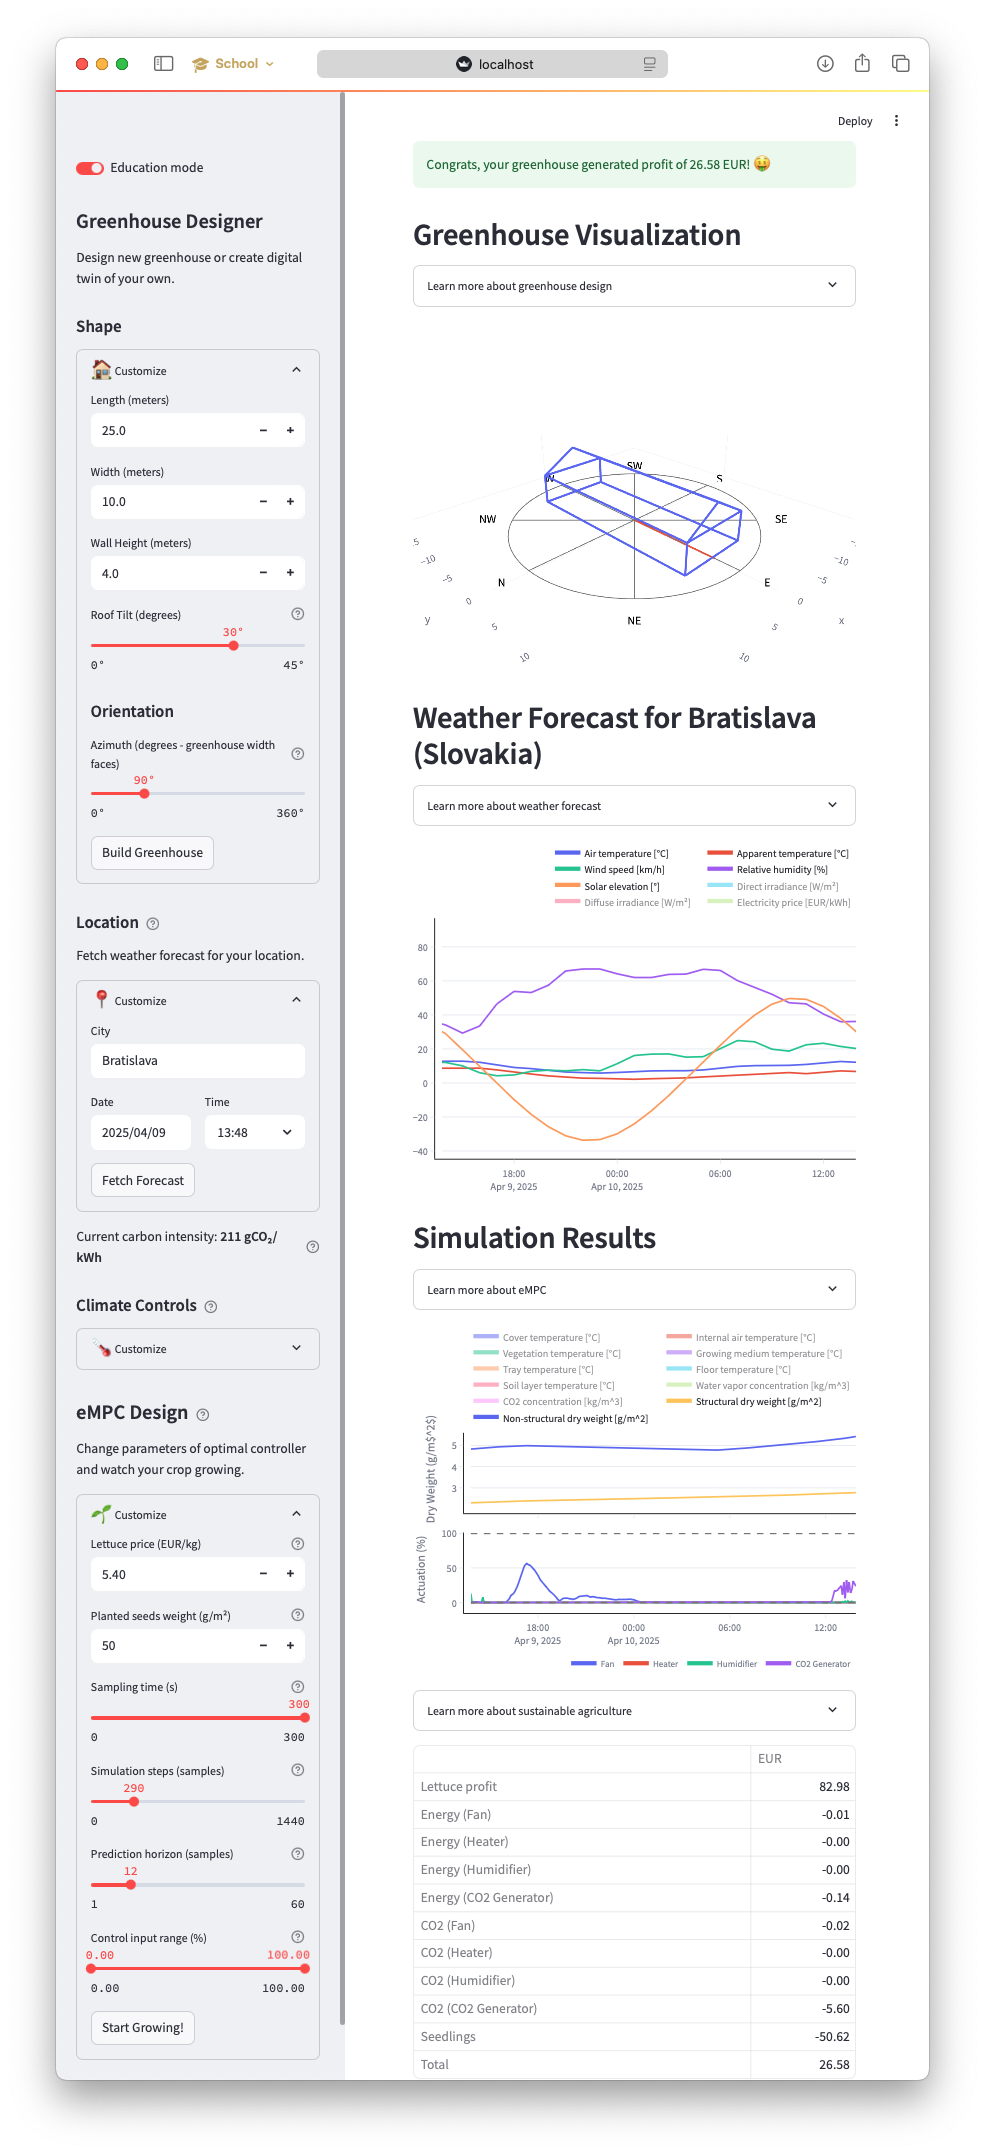
\includegraphics[width=\linewidth, trim=50 50 20 50]{figures/webpage.png}
    \caption{Education web interface. The sidebar ---  toggle to enable educational content, customization layers; the main window --- greenhouse structure, orientation, weather forecast, simulation results, and cost-profit analysis. The app is available at \url{https://ecompc4greenhouse.streamlit.app}.}\label{fig:web}
\end{figure}
The optimization and simulation are carried out using CasADi~\cite{Andersson2019} for modeling and discretizing the Nonlinear Economic MPC problem, while the IPOPT solver~\cite{Wachter2006} handles the optimization. These tools enable computationally efficient and scalable dynamic simulations of the greenhouse control system.

The proposed web application offers an accessible, interactive platform for teaching modern control concepts in a realistic setting. By combining simulation, real-time visualization, and economic-environmental trade-offs, it supports active learning and system-level thinking. At our institute, the tool could be integrated into several courses. At the bachelor level, it would complement the \textit{Vertical Project} course, where students work in teams on assignments involving our laboratory smart greenhouse. The app would help them simulate and test control strategies before applying them experimentally, enhancing their understanding of system dynamics.

\begin{table}
    \centering
    \caption{Performance comparison: NEMPC {vs. } no control.}\label{tab:comparison}
    \setlength{\tabcolsep}{4pt} % Reduce the column separation
    \begin{tabular}{lS[table-format=3.2]S[table-format=4.2]S[table-format=4.2]}
        \toprule
        \textbf{Parameter}  & {No control} & {NEMPC (\coo)} & {NEMPC (\$)} \\
        \midrule
        Lettuce profit      & 834.01       & 4459.57        & 4979.23      \\
        Energy (Fan)        & 0.00         & -0.34          & -0.36        \\
        Energy (Heater)     & 0.00         & -59.30         & -109.66      \\
        Energy (Humidifier) & 0.00         & -1.79          & -2.23        \\
        Energy (\coo\ Gen.) & 0.00         & -763.22        & -794.75      \\
        Energy (Solver)     & 0.00         & -0.001         & -0.001       \\
        \coo\ (Fan)         & 0.00         & -0.79          & -0.83        \\
        \coo\ (Heater)      & 0.00         & -158.51        & -378.51      \\
        \coo\ (Humidifier)  & 0.00         & -3.90          & -5.78        \\
        \coo\ (\coo\ Gen.)  & 0.00         & -2521.36       & -2705.12     \\
        \coo\ (Solver)      & 0.00         & -0.003         & -0.004       \\
        \midrule
        \textbf{Total}      & 834.01       & 950.36         & 981.99       \\
        \bottomrule
    \end{tabular}
\end{table}

\section{System Validation and Performance Analysis}
We analyze the behavior of the greenhouse under varying actuation, integrating climate data from a third-party API\@. Our analysis consists of two parts: first examining the influence of individual actuators on plant growth, and then evaluating the overall performance of the NEMPC algorithm compared to a no-control scenario.

To understand actuator influence on plant growth, we conducted simulations under a mild climate of Bratislava (Slovakia) on the 11\textsuperscript{th} of October. Figure~\ref{fig:steps} illustrates the responses of structural dry weight (SDW) and non-structural dry weight (NSDW) to various actuations. Columns 1 and 3 reveal that ventilation and humidification have minimal impact on growth, though they positively affect convection and energy transfer. Column 2 shows that intense heating facilitates the conversion of NSDW to SDW\@. Most significantly, column 4 demonstrates that \coo\ enrichment substantially enhances non-structural plant growth.
\begin{figure}
    \centering
    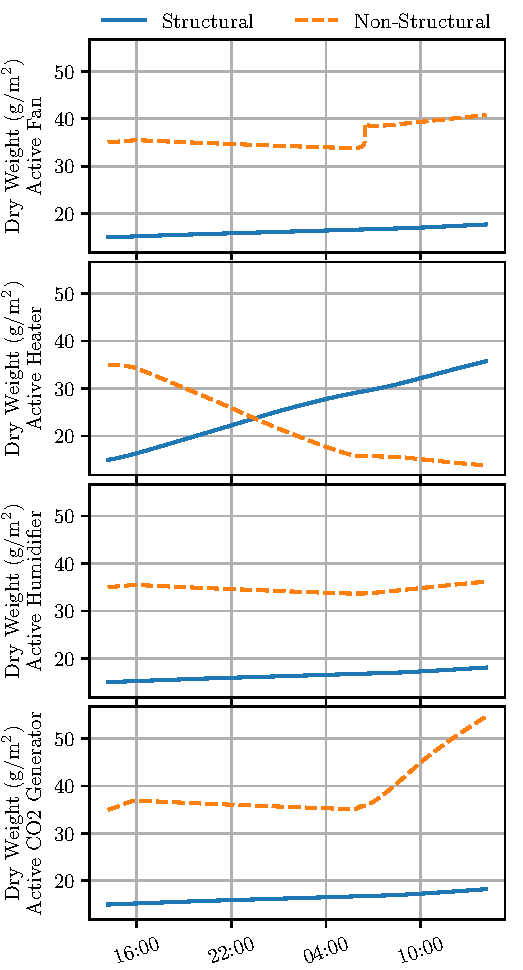
\includegraphics[]{figures/step_response-outputs-2024-10-11_2024-10-26-120s.pdf}
    \caption{Responses of structural and non-structural dry weight on step changes from off to maximum in following actuations from the left to the right: ventilation, heating, humidification, and \coo\ enrichment, no step made.}\label{fig:steps}
\end{figure}

To evaluate the NEMPC algorithm's performance, we conducted comparative simulations against a no-control scenario. The NEMPC was configured with both prediction and control horizons of 1 hour, running for 10,801 steps with a 120-second sampling time under the same climate conditions. Table~\ref{tab:comparison} presents the remarkable results: the proposed NEMPC increased crop yield by 435\% and improved profit by more than 14\% in just 15 days of growth. As shown in Fig.~\ref{fig:control}, the control strategy heavily utilizes the \coo\ generator while minimizing heater usage due to its high electricity consumption and the relatively mild autumn weather conditions.
Incorporating the social cost of carbon intensity in the NEMPC (\coo) cost function leads to a 15\% reduction in \coo\ consumption as compared to NEMPC (\$), although it caused a 11\% decrease in plant growth and 3\% decrease in profit when compared to a scenario where the social cost of \coo\ was not minimized. This highlights a trade-off between economic output and the carbon intensity of the energy sources. While farmers may prioritize economic gains, the environmental impact of production deserves careful consideration.
\begin{figure}
    \centering
    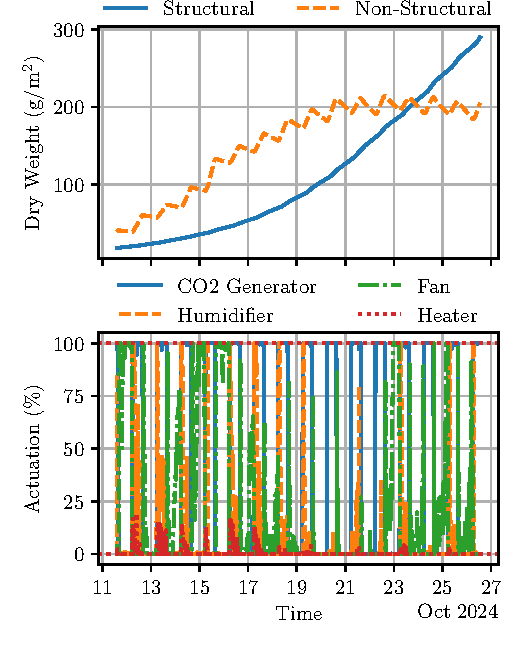
\includegraphics[width=\linewidth]{figures/greenhouse_control-mpc_co2-N_30-steps_10801.pdf}
    \caption{16 days of simulation display periodic utilization of CO\textsubscript{2} generator during the day. The heater is used mostly during initial growth phase. Both fan and humidifier are used extensively due to lower cost, mixing the humid air inside the greenhouse.}\label{fig:control}
\end{figure}

\section{Educational Framework Evaluation}
To assess the educational impact of this work, we conducted a survey among students who interacted with the application (Fig.~\ref{fig:feedbackPC}). The survey measured the participants prior knowledge and their learning outcomes in four key areas: mathematical modeling, optimal process control, economic process control, and MPC\@. Results from 13 responses reveal varying levels of initial expertise levels in modeling and process control, with self-ratings from novice to expert. Despite this variation, the application  proved educationally beneficial across all experience levels.

\begin{figure}
    \centering
    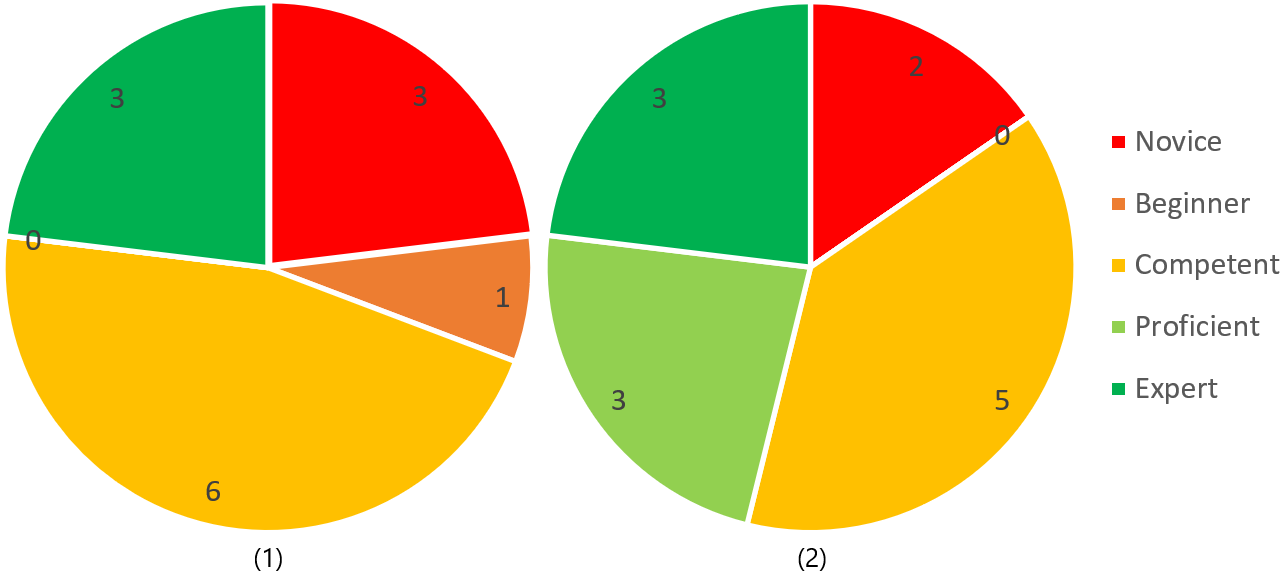
\includegraphics[width=\linewidth]{figures/feedbackPC.png}
    \caption{Self-reported familiarity with the topic prior to (1) and following (2) the experience.}\label{fig:feedbackPC}
\end{figure}

\paragraph{Low-Skilled Users}
Participants with minimal prior knowledge reported moderate improvements in understanding mathematical modeling, optimal control, and economic control, with a strong positive impact noted for MPC.\@ These results suggest that the framework is accessible to beginners and helps building foundational knowledge.

\paragraph{High-Skilled Users}
More experienced participants rated the application as highly beneficial in all categories. They noted substantial improvements in their understanding of complex control techniques, particularly in mathematical modeling and MPC, validating the educational potential of the framework for users with advanced backgrounds.

\paragraph{General Feedback}
Qualitative feedback from participants highlights the broader potential of the application. With additional information, the tool could be used by a broader audience, including industrial farmers, to design and optimize greenhouse placement in practical settings. This points to the dual benefit of the application: it not only enhances student learning but could also have real-world applicability in sustainable greenhouse design.

The proposed framework effectively supports educational objectives across a spectrum of learners, from beginners to advanced students. At the master's level, it enhances courses such as \textit{Automatic Control Theory}, \textit{Model Predictive Control}, and \textit{Modelling in the Process Industry} by allowing students to experiment with tuning horizons, constraints, cost functions, and explore how physical parameters affect model and control performance. This hands-on exploration strengthens their ability to connect theoretical concepts with real-world process dynamics.

Beyond educational contexts, the framework can be adapted for broader applications, providing valuable insights into the design and optimization of sustainable greenhouse systems. The combination of accessibility for students and depth for practical design considerations makes it a versatile tool that bridges the gap between academic learning and practical implementation in sustainable agriculture.

\section{Conclusion}
This study introduces a framework that combines the Nonlinear Economic Model Predictive Control with a detailed mathematical model to control the greenhouse climates, aiming to optimize lettuce growth. The provided framework utilizes real-time weather forecasts and carbon intensity data, to adjust the environmental conditions, improving crop yields, energy efficiency, and reducing \coo\ emissions.
%
The main contribution of this work is the educational tool helping students to understand not only the control theory but also to connect it with practical, real-world challenges. Through a user-friendly web-based platform, students can engage with advanced control theories while exploring the complexity of balancing economic goals and sustainability.
%
Student feedback has proven that the framework helps both beginning and advanced automatic control students to deepen their understanding of modeling, process control, and MPC techniques. Future work will focus on including other automatic control approaches to enrich the learning experience further.

\bibliographystyle{IEEEtran}
\bibliography{main}

\end{document}